\documentclass[midterm]{sparreport}

\title{Classifying GPU Workloads via Always-Available Telemetry for AI Compute Governance}
\author{
  \textbf{Sabiha Tajdari}\\
  University of Virginia\\
  \texttt{jvx2tt@virginia.edu}
  \and
  \textbf{Robi Rahman}\\
  Machine Intelligence Research Institute\\
  \texttt{robi@intelligence.org}
}
\sparround{Spring 2026}

\usepackage{booktabs}

\begin{document}
\maketitle

\begin{abstract}
Hardware-enabled governance of AI compute requires the ability to distinguish ML training from other GPU workloads.
We show that always-available Tier~1 NVML telemetry---GPU utilization, power draw, memory usage, and NVLink traffic, collected at zero runtime overhead---is sufficient for this task.
Using 73~statistical features extracted from 80~workload runs on NVIDIA A100 and H100 GPUs, a Random Forest classifier achieves 100\% binary accuracy (training vs.\ non-training) and 95.6\% accuracy across 15~workload types.
We design six adversarial edge cases that attack specific feature subsets; the hardest (frozen-backbone training) lies only $L_2=0.86$ from inference in feature space.
No single telemetry signal distinguishes all cases; a joint feature vector spanning utilization, power, timing, and NVLink counters is necessary and sufficient.
\end{abstract}

\keywords{GPU telemetry \and workload classification \and AI governance \and adversarial robustness}

\section{Introduction}

AI compute governance proposals increasingly rely on the ability to verify what workloads run on regulated hardware~\cite{aarne2024secure}.
Existing profiling tools such as NVIDIA Nsight Compute can fingerprint GPU workloads but impose 1{,}200--5{,}300\% runtime overhead~\cite{xu2026wave}, making continuous deployment impractical.
We ask: \emph{can zero-overhead, always-available GPU telemetry reliably distinguish ML training from other workloads---even when an operator adversarially disguises the workload?}

We make four contributions:
(1)~a telemetry-based classifier achieving 100\% binary and 95.6\% 15-class accuracy using only Tier~1 NVML metrics at zero overhead;
(2)~systematic adversarial robustness testing with six evasion strategies;
(3)~a demonstration that joint feature vectors are necessary---no single signal suffices; and
(4)~a concrete recommendation of which metrics a Hardware-Enabled Mechanism (HEM) should monitor.

\section{Related Work}

WAVE~\cite{xu2026wave} fingerprints LLM \emph{inference} workloads using nine Nsight Compute performance counters, achieving 87--93\% model identification accuracy.
However, it targets inference rather than training and requires expensive Tier~3 profiling.
Differential Architecture~\cite{anonymous2026differential} characterizes hardware bottleneck regimes (compute-bound, memory-bound, cache-bound) across GPU workload classes but does not build classifiers or test adversarial evasion.
ShadowScope~\cite{jackowski2025shadowscope} validates GPU kernel behavior via CUPTI performance counters for governance applications.
No prior work addresses training-specific detection combined with adversarial robustness using zero-overhead telemetry.

\section{Methods}

\paragraph{Hardware and telemetry.}
Experiments run on 2$\times$ NVIDIA H100 80\,GB HBM3 GPUs with NVLink~4.0, validated on A100 SXM4.
We poll \texttt{pynvml} at 100--200\,ms intervals, capturing nine raw signals: GPU utilization, memory utilization, memory used, power draw, temperature, SM clock, memory clock, and PCIe TX/RX bandwidth.
This Tier~1 telemetry imposes zero runtime overhead.

\paragraph{Feature extraction.}
From each run's time series we compute 73~aggregate features: mean, standard deviation, coefficient of variation (CV), skewness, kurtosis, autocorrelation at lag~1, and the 5th/95th percentiles for each signal.

\paragraph{Workloads.}
We collect 80~runs across 15~workload types spanning five categories: ML training (ResNet, BERT, GPT-2, MLP in FP32 and AMP, single-GPU and DDP), ML inference (ResNet-50), scientific HPC (3D FFT, N-body), crypto mining (Ethash proxy), rendering (Monte Carlo ray tracing), and idle baseline.

\paragraph{Classifiers.}
We train Random Forest, Logistic Regression, and SVM-RBF classifiers on four tasks: binary (training vs.\ rest), three-way (training/inference/other), 7-category, and 15-class.
Evaluation uses stratified group $k$-fold cross-validation grouped by run ID to prevent data leakage.

\paragraph{Adversarial edge cases.}
We design six workloads that attack specific classifier features:
(1)~phantom training (inference + fake allreduce),
(2)~silent training (\texttt{no\_sync} suppresses NVLink),
(3)~sparse sync (gradient accumulation $\times$16),
(4)~mining-like inference (high-batch, max utilization),
(5)~frozen-backbone training (head-only fine-tuning), and
(6)~low-intensity training (tiny model, small batch).

\section{Results}

\subsection{Clean-Data Classification}

On 80 runs (21{,}617 telemetry rows, 73 features), the Random Forest achieves 100\% binary accuracy (training vs.\ rest), 100\% three-way accuracy, 98.75\% on 7~categories, and 95.6\% on all 15~workload labels.
Logistic Regression matches the binary and three-way results.
Sliding-window evaluation at 30\,s windows also achieves 100\% binary accuracy.
The top discriminating features are GPU utilization CV (19\% importance), SM clock standard deviation (15\%), and memory features (24\% combined); see \cref{fig:classifier}.
A simple decision rule---GPU utilization CV $> 30\%$---correctly identifies all training runs in our dataset.

\begin{figure}[t]
  \centering
  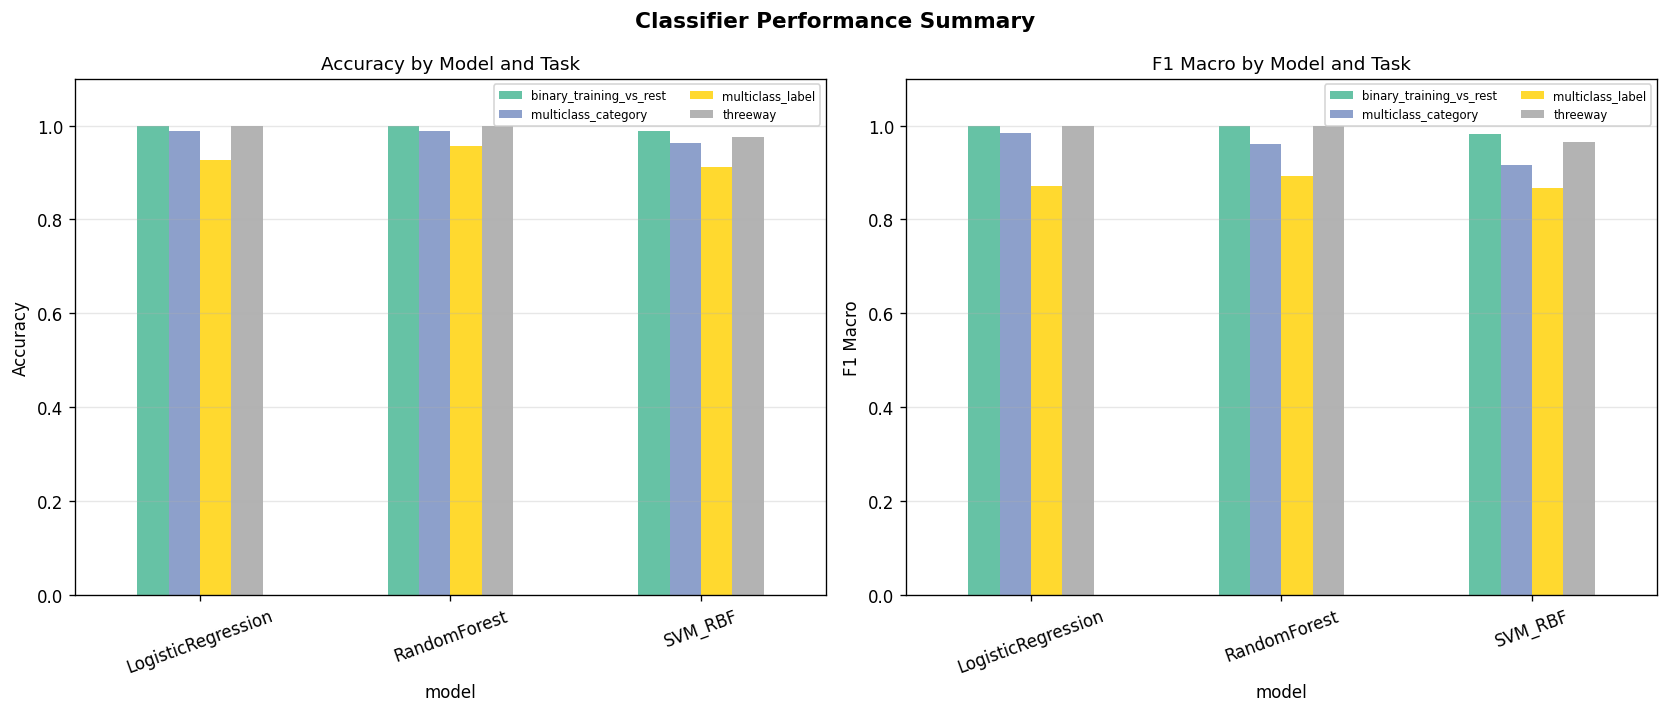
\includegraphics[width=\columnwidth]{figures/classifier_summary.png}
  \caption{Classifier accuracy across four tasks. Random Forest and Logistic Regression achieve 100\% on binary and three-way classification.}
  \label{fig:classifier}
\end{figure}

\subsection{Adversarial Robustness}

Six adversarial workloads probe classifier boundaries (\cref{fig:edgecases}).
The hardest case is EC-5 (frozen backbone): with only 5{,}120 bytes of gradient payload, its NVLink and memory signatures are indistinguishable from inference ($L_2 = 0.86$).
The easiest to detect is EC-4 (mining-like inference, $L_2 > 7.0$) due to its anomalous power draw (213\,W vs.\ 91\,W baseline).
Critically, no single feature separates all cases.
EC-1 defeats NVLink-only classifiers; EC-2 defeats them from the opposite direction; EC-6 falls within the inference range on \emph{every} individual feature.
Only the joint vector---forward time, backward time, allreduce time, NVLink bytes, utilization, and power---correctly classifies all eight workloads (six adversarial plus two baselines).

\begin{figure}[t]
  \centering
  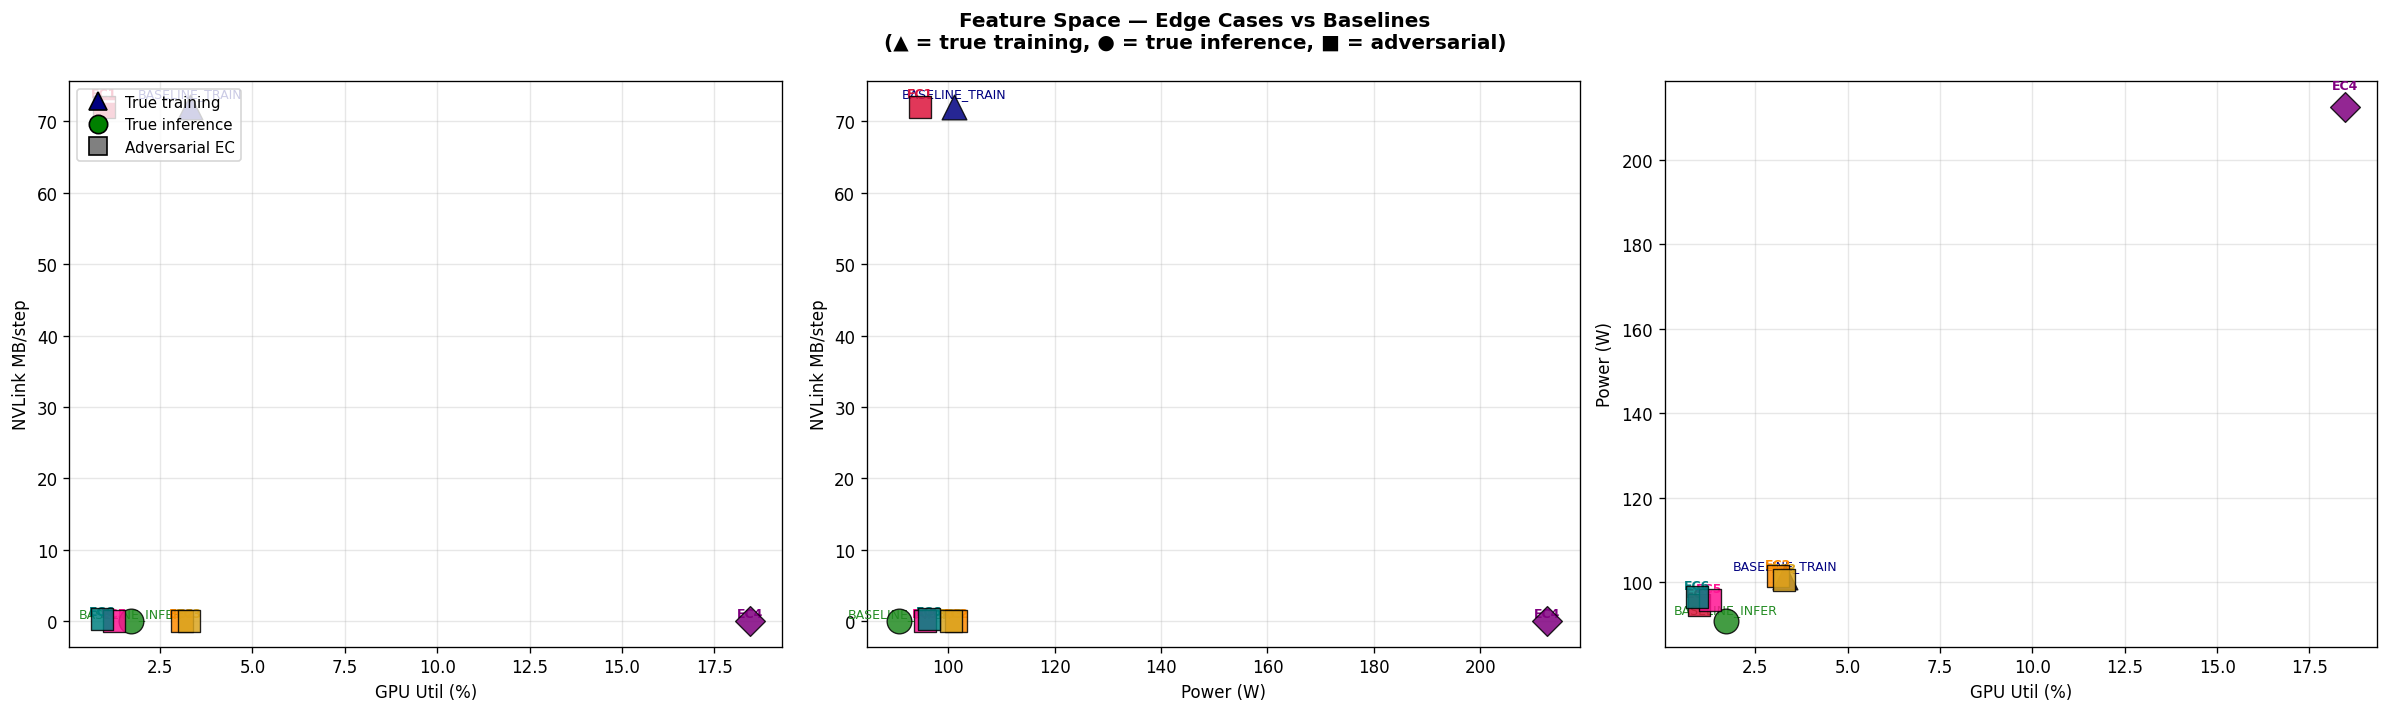
\includegraphics[width=\columnwidth]{figures/edge_cases_feature_scatter.png}
  \caption{Adversarial edge cases in feature space. EC-5 (frozen backbone) is nearest to inference ($L_2 = 0.86$). No single 2D projection separates all cases.}
  \label{fig:edgecases}
\end{figure}

\section{Discussion}

The GPU microarchitecture acts as an \emph{involuntary witness}: the physical constraints of computation impose characteristic signatures that cannot be simultaneously falsified across all observable dimensions.
An adversary can suppress NVLink traffic (EC-2) or mimic inference timing (EC-5), but doing both while maintaining training functionality requires accepting significant throughput or accuracy penalties.

The frozen-backbone case (EC-5) is particularly instructive: it shows that a governance system must monitor backward-pass timing, not just utilization or NVLink volume.
This has a concrete design implication for HEMs: logging forward and backward pass durations at the framework level, alongside Tier~1 NVML counters, would close the remaining detection gap.

\paragraph{Limitations.}
All experiments use a single two-GPU node; multi-node distributed training may distribute the allreduce signature differently.
Tier~1 NVML cannot observe kernel-level instruction mix, unlike WAVE's Tier~3 profiling.
The adversarial strategies are researcher-designed; a real-world adversary with full classifier knowledge may find additional evasion vectors.

\paragraph{Future work.}
We plan cross-GPU generalization experiments on a third architecture (RTX~5070~Ti), physical side-channel validation via wall-power measurement, and an expanded adversarial evaluation.

\section{Conclusion}

Always-available Tier~1 NVML telemetry can detect ML training with 100\% binary accuracy under clean conditions and identify the hardest adversarial evasion (frozen backbone, $L_2 = 0.86$).
No single feature suffices; joint feature vectors are necessary.
These results provide an empirical foundation for hardware-enabled monitoring: a HEM logging GPU utilization, power, memory, and NVLink traffic at 100\,ms intervals would be sufficient for training detection at zero runtime overhead.

\bibliographystyle{plain}
\bibliography{references}

\end{document}
